\documentclass[10pt,a4paper]{article}
\usepackage[margin=0.8in]{geometry}
\usepackage[T1]{fontenc}
\usepackage{mathptmx}
\usepackage{graphicx}
\usepackage{booktabs}
\usepackage{caption}
\usepackage{microtype}
\usepackage[hidelinks]{hyperref}
\captionsetup{font=small,labelfont=bf,skip=3pt}
\setlength{\parskip}{3pt}
\setlength{\parindent}{0pt}
\renewcommand{\arraystretch}{1.05}

\title{\vspace{-1.2cm}\textbf{Learned Page Replacement Under a Workload Shift}\\[2pt]
\large CSE-307 Operating Systems, Part B Term Paper (Track 1)}
\author{Sayed Md Shafiqul Islam \\ ID: 202414011 \quad Section A \quad CSE 24}
\date{4 October 2026}

\begin{document}
\maketitle
\vspace{-0.8cm}

\section{Problem Framing}
Page replacement decides which resident page to evict when a reference faults and memory is full. FIFO and LRU are fixed rules: FIFO ignores usage, and LRU assumes that the recent past predicts the near future \cite{silberschatz}. Belady's optimal policy (OPT) evicts the page whose next use is farthest away. It needs future knowledge, so it is only a lower bound on faults that online policies are measured against \cite{belady,mattson}. Real workloads change phase, so a policy that suits one phase can suit the next one badly.

This paper asks two questions. (1)~Can a small learned model that predicts page reuse from simple features beat FIFO and LRU? (2)~What happens to each policy, including the learned one, when the access pattern shifts half-way through a run? The learned component is deliberately lightweight (a depth-4 decision tree), in the spirit of ML-driven caching work such as LeCaR \cite{lecar}.

\section{Implementation}
All code is Python~3 with NumPy \cite{numpy} and scikit-learn \cite{sklearn}. A single simulator replays a page-reference string against $F$ frames, and each policy only supplies a victim-selection rule.
\begin{itemize}\setlength{\itemsep}{0pt}
\item \textbf{FIFO}: evicts the page loaded earliest. \textbf{LRU}: evicts the least recently referenced page. \textbf{OPT}: evicts the resident page with the farthest next reference, computed from a precomputed next-use array.
\item \textbf{Correctness checks}: on the textbook reference string with 3 frames \cite{silberschatz} the simulator reproduces 15 (FIFO), 12 (LRU) and 9 (OPT) faults, and a test confirms that OPT never has more faults than any other policy on the synthetic traces.
\item \textbf{Learned policy.} At every eviction, each resident page is described by four features an OS could keep as page metadata: \emph{recency} (accesses since last use), \emph{frequency} (uses in the last 256 accesses), \emph{age in memory}, and \emph{last reuse gap}. A decision tree (max depth 4, min leaf 20) predicts whether the page will be referenced again within $H{=}64$ accesses. The page with the lowest predicted reuse probability is evicted, with ties broken by recency.
\item \textbf{Two variants.} \emph{Learned-static} is trained offline on three pre-shift traces (different seeds from all test traces) and then frozen. \emph{Learned-adaptive} starts from the same model and retrains every 1000 accesses on the most recent 6000 labelled decisions. A decision is labelled only $H$ accesses after it was made, so no future information leaks into training.
\end{itemize}

\section{Experimental Setup}
Each trace has 20{,}000 references over $V{=}256$ virtual pages, with a deliberate shift at reference 10{,}000.
\textbf{Phase~1 (locality-heavy/sequential):} 70\% of references go to a 20-page hot set with Zipf weights, and 30\% are a cyclic sequential scan over the other 236 pages. The scan pollutes recency-based policies.
\textbf{Phase~2 (random/bursty):} uniform-random references interleaved with bursts of 10--40 references to a random 8-page region (about 40\% of references fall inside bursts).
The main configuration uses $F{=}32$ frames and 10 random seeds; memory sizes 16, 32 and 64 are also tested. Hits and faults are counted separately for each half. Results are mean $\pm$ standard deviation over seeds. Everything is reproducible with \texttt{python run\_experiments.py}.

\section{Results}
\begin{table}[h]
\centering\small
\caption{Hit ratio and faults per 10{,}000 references before/after the shift ($F{=}32$, 10 traces). ``Drop'' is the loss in hit ratio in percentage points (pp); ``Gap'' is the distance to OPT after the shift.}
\label{tab:main}
\begin{tabular}{lcccccc}
\toprule
Policy & Hit\% before & Hit\% after & Drop (pp) & Faults before & Faults after & Gap (pp) \\
\midrule
FIFO & 52.7 $\pm$ 0.5 & 38.3 $\pm$ 1.1 & 14.4 & 4732 & 6171 & 20.8 \\
LRU & 60.5 $\pm$ 0.5 & 38.4 $\pm$ 1.2 & 22.1 & 3946 & 6158 & 20.7 \\
OPT & 71.1 $\pm$ 0.3 & 59.1 $\pm$ 0.7 & 12.0 & 2890 & 4086 & 0.0 \\
Learned-static & 67.3 $\pm$ 0.4 & 34.2 $\pm$ 1.2 & 33.1 & 3267 & 6578 & 24.9 \\
Learned-adaptive & 69.2 $\pm$ 0.5 & 36.0 $\pm$ 1.0 & 33.2 & 3080 & 6396 & 23.1 \\
\bottomrule
\end{tabular}

\end{table}

\begin{figure}[h]
\centering
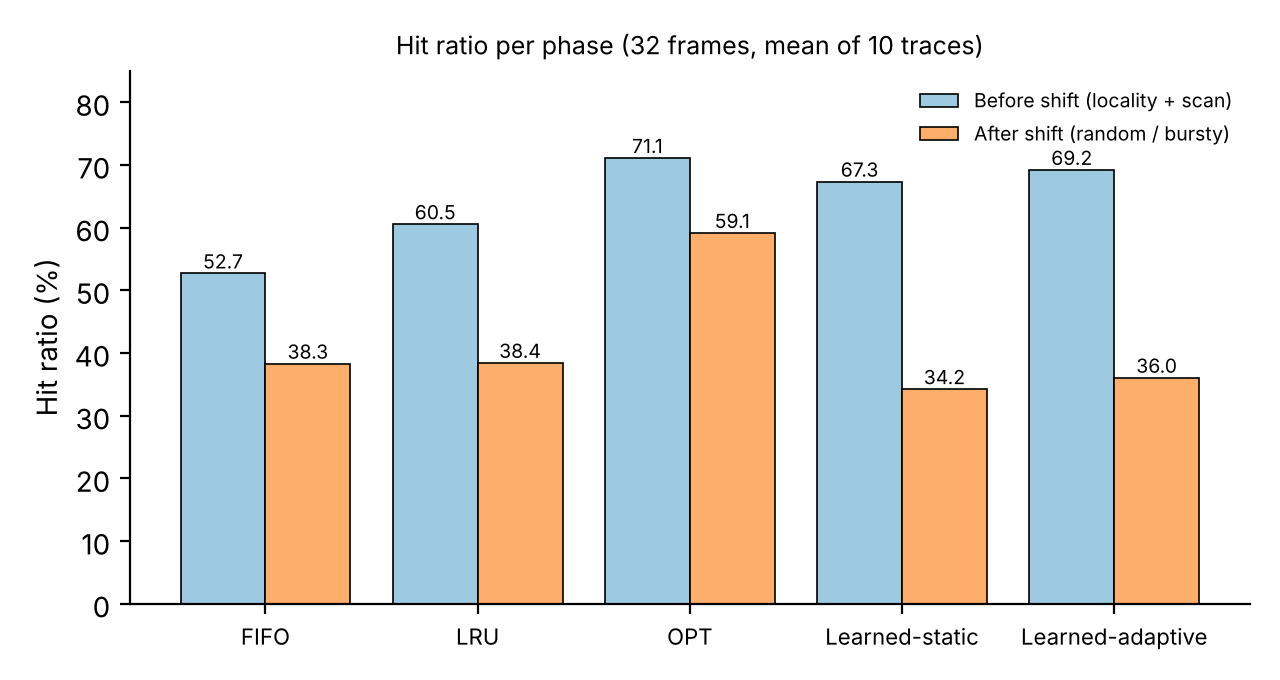
\includegraphics[width=0.49\linewidth]{../results/fig_phase_hit_ratio.png}\hfill
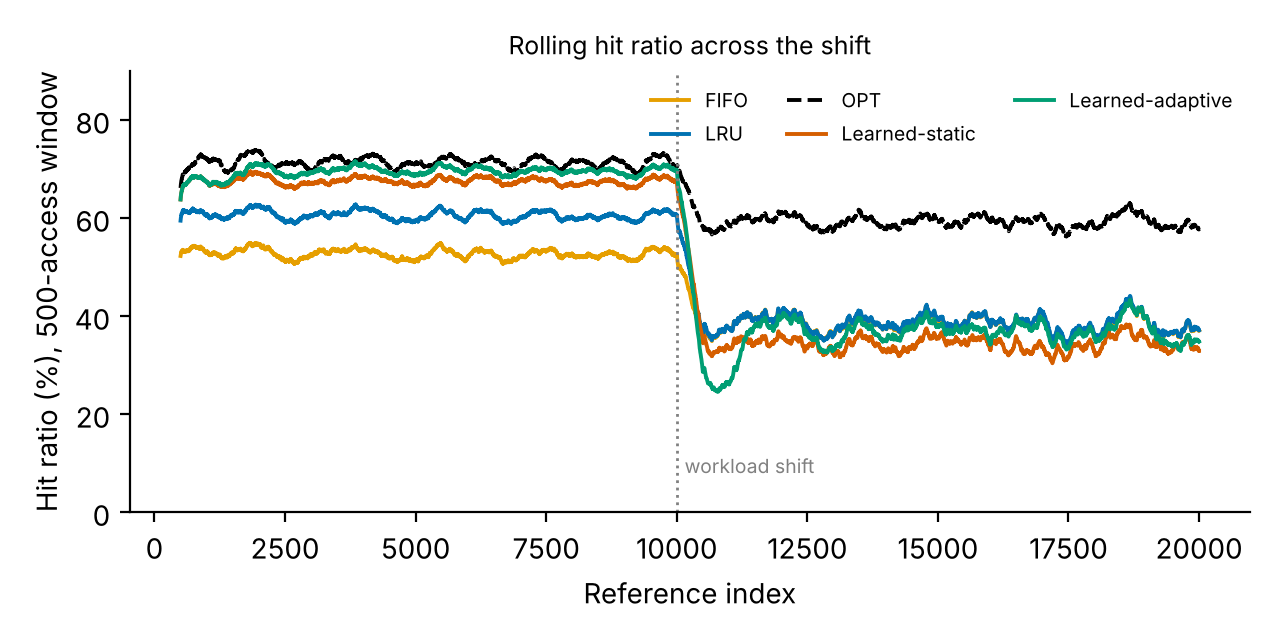
\includegraphics[width=0.49\linewidth]{../results/fig_rolling_hit_ratio.png}
\caption{Left: hit ratio per phase. Right: 500-access rolling hit ratio averaged over 10 traces; the dotted line marks the shift.}
\label{fig:main}
\end{figure}

Before the shift the learned policies clearly win among online policies: 67.3\% (static) and 69.2\% (adaptive) against 60.5\% for LRU and 52.7\% for FIFO, within 3.8 and 1.9 pp of OPT's 71.1\%. After the shift the picture reverses. FIFO and LRU both fall to about 38.4\%, while Learned-static falls to 34.2\% and Learned-adaptive to 36.0\%, so both learned variants end \emph{below} LRU. The learned policies suffer the largest drop (about 33 pp), against 22.1 pp for LRU, 14.4 pp for FIFO and 12.0 pp for OPT. Figure~\ref{fig:main} (right) shows the adaptive variant falling to roughly 25\% right after the shift before recovering to the level of LRU within about 2000 references.

\begin{figure}[h]
\centering
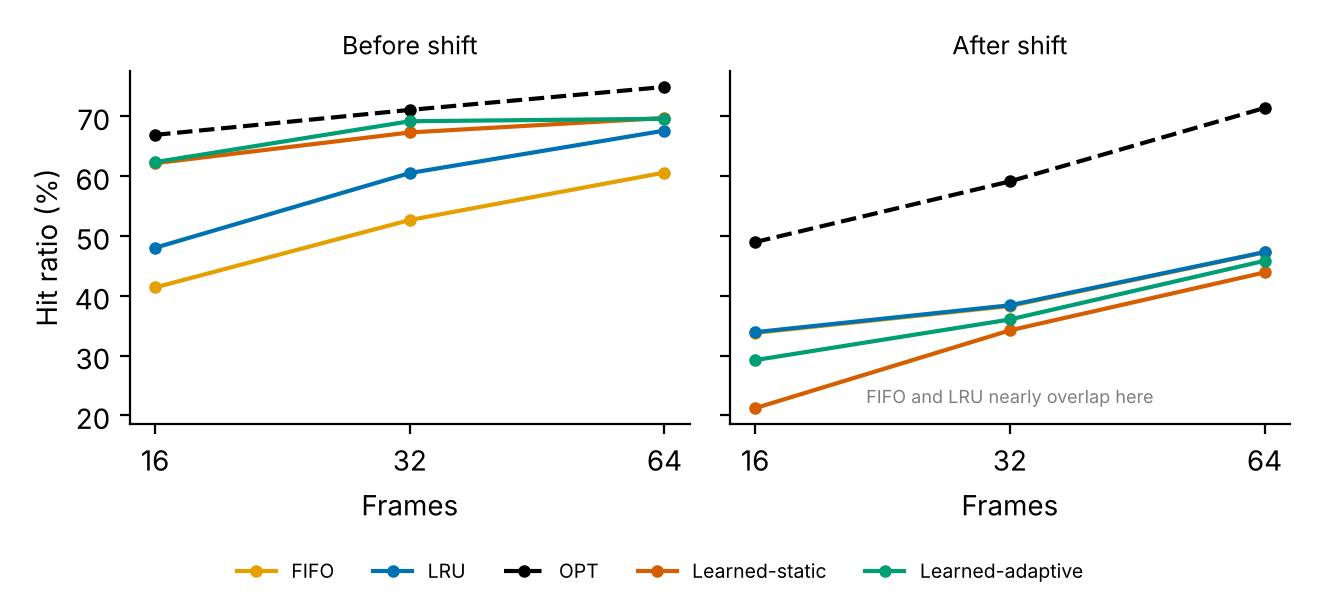
\includegraphics[width=0.78\linewidth]{../results/fig_frame_sweep.png}
\caption{Hit ratio vs.\ number of frames, before and after the shift.}
\label{fig:sweep}
\end{figure}

Memory size matters (Figure~\ref{fig:sweep}). With 16 frames the frozen model is badly hurt after the shift (21.2\% against 33.9\% for LRU), whereas with 64 frames the gap narrows (43.9\% against 47.3\%). OPT stays far ahead after the shift at every size, so a large part of the available benefit is future knowledge that no online policy has.

\section{Analysis: What Changed Under the Shift}
\textbf{Why the learned policy wins first.} The trained tree is almost entirely a frequency rule (99.4\% of feature importance): pages used at least twice in the recent window are kept, and pages seen once are evicted first. In phase~1 this is exactly right. Scan pages are touched once per cycle and are useless, but they flood an LRU list and push out warm hot pages. Frequency recognises scan pages and protects the hot set, which is why the learned policy beats LRU there.

\textbf{Why it degrades the most.} The model learned a property of the old workload (``high frequency means reuse soon''), and that property stops being true. After the shift, most pages are random and have frequency near one, so decisions fall back to recency, which is LRU-like. Pages from finished bursts, however, keep a high frequency count and are still protected. We measured this directly (10 traces, post-shift): on average 12.2 of the 32 frames hold pages the model rates as likely to be reused although they have not been touched for over 100 accesses, and the frozen model evicts a page that is needed again within 16 accesses in 10.8\% of evictions, against 4.9\% for LRU. It is plausible that the first accesses of a new burst, which still have frequency one, are evicted too early, but we did not isolate this effect. Stale frequency information of this kind is a known weakness of frequency-based policies.

\textbf{Why FIFO and OPT ``drop'' less.} FIFO's smaller drop (14.4 pp) is mostly a floor effect: it was already the weakest policy before the shift, and after the shift it is as good as LRU. OPT's 12.0 pp drop shows that part of the loss is unavoidable, because random references offer less reusable locality than the hot set did. The remaining gap to OPT is the cost of not knowing the future, and it is about 21 pp for FIFO/LRU and 23--25 pp for the learned variants.

\textbf{Does adapting help?} Partly. Retraining recovers 1.8 pp over the frozen model after the shift (36.0\% vs.\ 34.2\%) and 8.7 pp over LRU before it, but it does not beat LRU after the shift. It learns from labels that arrive $H$ references late, and its training window still contains pre-shift decisions, hence the dip in Figure~\ref{fig:main}. Retraining every 500, 1000 and 2000 references gives post-shift hit ratios of 36.5\%, 36.0\% and 33.6\%, so faster adaptation helps but only modestly.

\section{Limitations and Conclusion}
The traces are synthetic, with a single shift and hand-chosen parameters, so the absolute numbers will differ on real traces and the ranking after the shift depends on how bursty phase~2 is. The model is a small tree evaluated in a simulator, and its run-time cost and metadata overhead inside a kernel are not modelled. OPT is an offline reference only.

In summary, a tiny learned eviction rule beat LRU by 7--9 pp while the workload matched its training data, but it also lost the most when the pattern changed, finishing 2--4 pp \emph{below} LRU after the shift. Online retraining reduces the damage without removing it. The practical lesson is that a learned OS heuristic needs drift detection and a safe fallback (such as LRU), not just a good offline accuracy.

\begin{thebibliography}{9}\small
\bibitem{belady} L.~A. Belady, ``A study of replacement algorithms for a virtual-storage computer,'' \emph{IBM Systems Journal}, vol.~5, no.~2, pp.~78--101, 1966.
\bibitem{mattson} R.~L. Mattson, J.~Gecsei, D.~R. Slutz, and I.~L. Traiger, ``Evaluation techniques for storage hierarchies,'' \emph{IBM Systems Journal}, vol.~9, no.~2, pp.~78--117, 1970.
\bibitem{silberschatz} A.~Silberschatz, P.~B. Galvin, and G.~Gagne, \emph{Operating System Concepts}, 10th ed. Wiley, 2018.
\bibitem{lecar} G.~Vietri \emph{et al.}, ``Driving cache replacement with ML-based LeCaR,'' in \emph{Proc. USENIX HotStorage}, 2018.
\bibitem{sklearn} F.~Pedregosa \emph{et al.}, ``Scikit-learn: Machine learning in Python,'' \emph{J. Machine Learning Research}, vol.~12, pp.~2825--2830, 2011.
\bibitem{numpy} C.~R. Harris \emph{et al.}, ``Array programming with NumPy,'' \emph{Nature}, vol.~585, pp.~357--362, 2020.
\end{thebibliography}

\end{document}
